\documentclass[10pt]{report}
\usepackage{documento}
\usepackage{procesos}
\usepackage{verbatim} % comentarios
\title{Reporte}
\subtitle{Sistema Auxiliar para la revisión de Programas de Estudio}
\author{Ingeniería de Software}
\date{\today}

\begin{document}
\maketitle
\thispagestyle{empty}
\tableofcontents
\chapter{Descripción}
\section{Problemática}
En el proceso actual de la División de Innovación Academica de la Dirección de Educación Superior(DES), se identifico como área de oportunidad la elaboración y revisión de Programas de Estudio de las Unidades de Aprendizaje para la creación o rediseño de un Plan de Estudios. Debido a las siguientes situaciones:\\
\begin{itemize}
    \item Tiempo desperdiciado en la revisión de detalles innecesarios o información repetida, por ejemplo revisar que concuerden los creditos, las horas, los nombre de las Unidades de Aprendizaje, etc.
    \item Modificaciones a secciones ya aceptadas previamente, es decir que no necesitaban corregirse.
    \item Medio de comunicación externo.
    \item Estructura incorrecta del documento final, por ejemplo saltos de paginas incorrectos, tablas partidas, etc.
    \item Correcciones ignoradas.
    \item Revisiones incompletas o inexistentes por parte de las Unidades Académicas.
\end{itemize}
\begin{figure}[H]
	\centering
	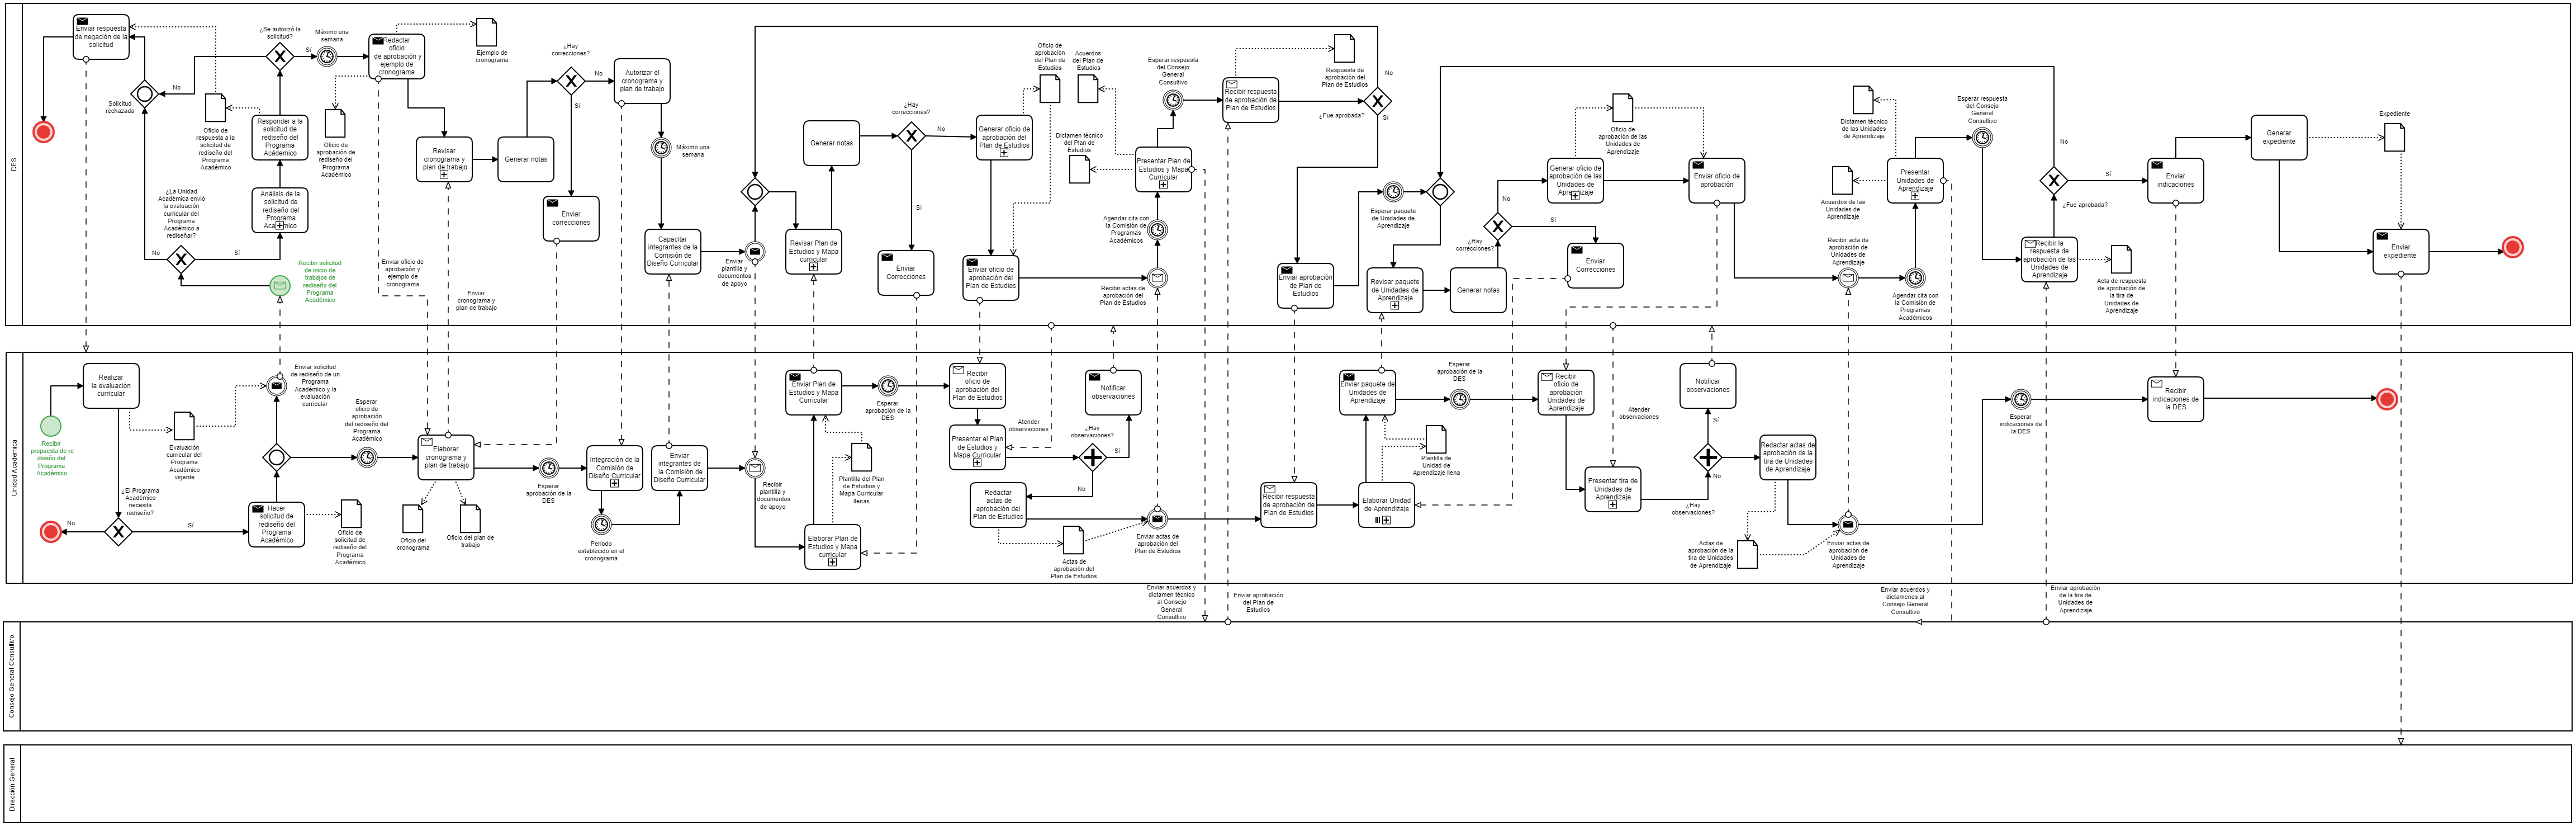
\includegraphics[width=0.9\linewidth]{images/Procesos/MacroProceso}
	\caption{Modelado del Negocio}
\end{figure}

\section{Solución}
La solución propuesta consiste en el desarrollo de un plataforma web, que asista en la elaboración y revisión de los Programas de Estudio de las Unidades de Aprendizaje.\\
\\
Se planteo tener un control de usuarios con jerarquia para cumplir con los protocolos establecidos, automatización de los datos obtenidos mediante formulas o reglas, realizar el registro y la revisión de manera seccionada permitiendo bloquear secciones ya aceptadas, generar automaticamente el documento final, guardar en una bitácora las correcciones relizadas a un documento durante todo el proceso.
\section{Objetivos}
Con la solución propuesta se busca minimizar las causas que se identificaron en la Problemática.\\
\\
Establecer el control de usarios para así tener un mayor control sobre los cambios y forzar el seguimiento del protocolo.\\
\\
Registrar y revisar de manera seccionada para poder ir bloqueando las que ya hayan sido aceptadas.\\
\\
Generar el documento de acuerdo a las platillas proporcionadas por la Dirección de Educación Superior.\\
\\
Calcular los datos que pueden ser obtenidos mediante otros y reutilizar la información ya registrada, evitando trabajo innecesario que son posibles fuentes de error.\\
\\
Guardar las correcciones señaladas a lo largo del proceso sobre un Porgrama de Estudios para así tener evidencia de las correcciones que debieron hacerse.
\include{modulos/Requerimientos}
\section{Arquitectura del Sistema}

\subsection{Aquitectura de conexión}


\begin{figure}[!h]
	\centering	
	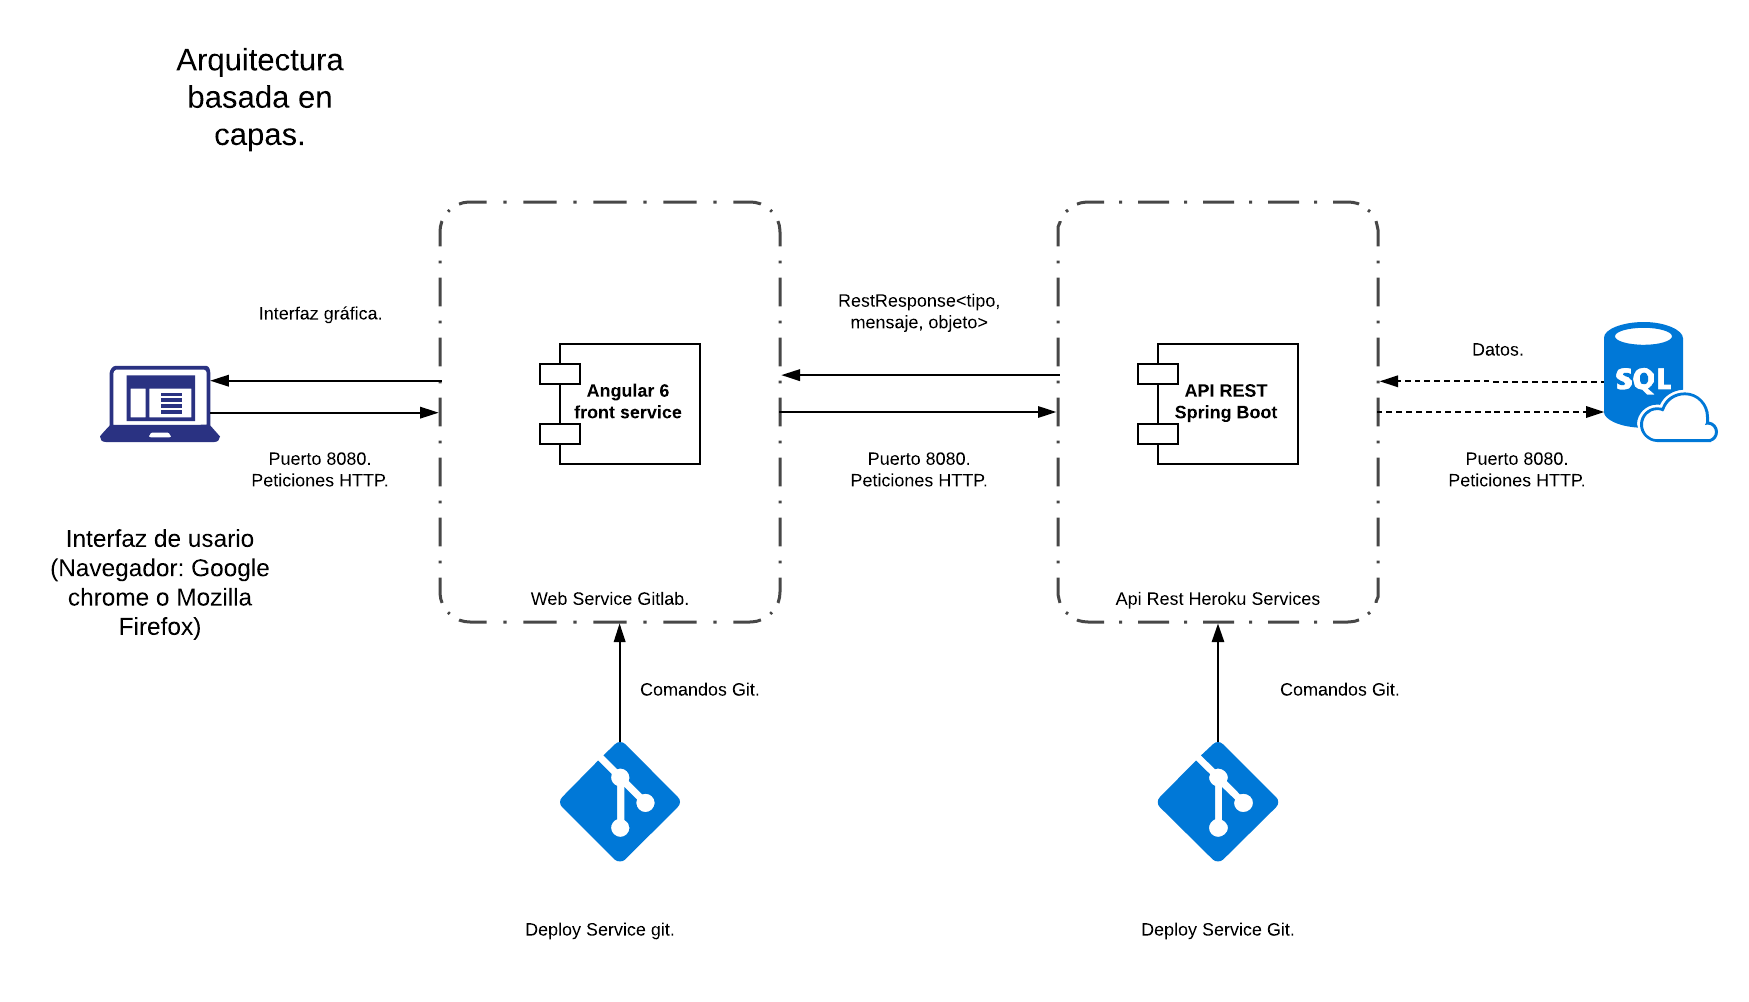
\includegraphics[width=0.8\linewidth]{images/Arquitectura/Blank_Diagram2.png}
	\caption{Representación gráfica de la conexión de servicios de la arquitectura del sistema.}
\end{figure}


La arquitectura del sistema propuesta es una arquitectura en capas, las cuales están definidas dentro de la figura 1. Está compuesta por:

\begin{itemsize}
	\item Una capa de presentación (funcionalidad relacionada con la interfaz de usuario), una capa de negocios (procesamiento de reglas de negocios) y una capa de datos (funcionalidad relacionada con el acceso a datos).

	\item La capa de interfaz utiliza el framework angular para la interpretación  de los eventos ocurridos en el navegador por parte del usuario, el sistema está guardado en un servidor que provee gitlab basado en node js. 

	\item La lógica del negocio se encuentra en un servidor que se encuentra alojado en los servidores de Heroku y está programado en java con el framework spring boot.
Para la base de datos se utilizó una basada en relaciones, ésta está alojada en Amazon web Service.
\end{itemize}


\subsection{Lista de peticiones}

Por convención, se utilizará las peticiones propias del protocolo HTTP: GET, POST, PUT, DELETE.

\subsection{Formas de recibir información}

La información se enviara a través de paquetes JSON.

Por parte del servidor tenemos que se enviará la información con la siguiente forma:

\begin{figure}[!h]
\centering
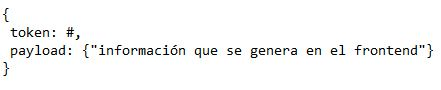
\includegraphics[width=0.7\linewidth]{images/Arquitectura/Captura.JPG}
\caption{Representación gráfica de la estructura por petición del frontend al backend}
\end{figure}


A continuación se definen los campos de la Figura 2:
\begin{itemize}
  \item token: Este campo hace referencia a la información necesaria del usuario que hace la petición \newline al servidor del backend.
  \item payload: Este campo hace referencia a la información principal de que será procesada por\newline el servidor del backend.
\end{itemize}


Por parte del back al frontend tenemos que la información se enviará con la siguiente estructura:

\begin{figure}[!h]
\centering
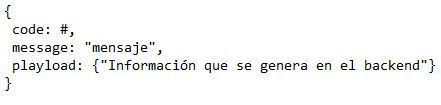
\includegraphics[width=0.7\linewidth]{images/Arquitectura/back.JPG}
\caption{Representación gráfica de la estructura por petición del backend al frontend}
\end{figure}

A continuación se definen los campos de la Figura 3:
\begin{itemize}
  \item code: Este campo es un número que el servidor del backend enviará para verificar si la información se procesó correctamente o hubo un error.
  \item message: Este campo es un mensaje que el servidor del backend enviará para verificar si la información se procesó correctamente o hubo un error. 
  \item payload: Este campo hace referencia a la información principal que fue recuperada de la base de datos y que será procesada por el servidor del frontend.
\end{itemize}


\include{modulos/Pruebas}
%----------- REQUERIMIENTOS --------
\chapter{Documento de Requerimientos}
\section{Macroproceso}
% -------------- TABLA PARA REQUERIMIENTOS FUNCIONALES ---------------- %
% Nomenclatura para la prioridad:
%	A - Alta
%	M - Media
%	B - Baja
\begin{table}[htbp!]
	\begin{requerimientos}
		\FRitem{RU1}{Autorizar el rediseño del Programa Académico}{El sistema permitirá aprobar la solicitud de rediseño del Programa Académico antes de elaborar el Plan de Estudios.}{M}{Origen}

		\FRitem{RU2}{Elaborar Plan de Estudios y Mapa Curricular}{El sistema debe permitir que la Unidad Académica llene los datos correspondientes del Plan de Estudios y Mapa Curricular enviadas por la DES.}{A}{Origen}

		\FRitem{RU3}{Enviar Plan de Estudios y Mapa Curricular}{El sistema debe permitir que la Unidad Académica envíe la propuesta del Plan de Estudios y Mapa Curricular a la DES para su revisión.}{A}{Origen}

		\FRitem{RU4}{Enviar correcciones del Plan de Estudios}{El sistema debe permitir que la DES genere y envie a la Unidad Académica correcciones del Plan de Estudios propuesto por ésta.}{A}{Origen}

		\FRitem{RU5}{Notificar aprobación de Plan de Estudios}{El sistema debe permitir notificar a la Unidad Académica la aprobación del Plan de Estudios.}{B}{Origen}

		\FRitem{RU6}{Enviar plantillas y documentos de apoyo para la elaboración de las Unidades de Aprendizaje}{El sistema debe permitir que la DES envie las plantillas y documentos de apoyo para elaborar las Unidades de Aprendizaje a la Unidad Académica.}{A}{Origen}

	\end{requerimientos}
    \label{tbl:}
\end{table}

\begin{table}[htbp!]
	\begin{requerimientos}

		\FRitem{RU7}{Elaborar Unidades de Aprendizaje}{El sistema debe permitir que la Unidad Académica llene la propuesta de las Unidades de aprendizaje enviadas por la DES. Pueden ser por paquetes o por semestre.}{A}{Origen}

		\FRitem{RU8}{Enviar paquetes de Unidades de Aprendizaje}{El sistema debe permitir que la Unidad Académica envíe la propuesta de las Unidades de Aprendizaje llenas por paquetes a la DES para su revisión.}{A}{Origen}

		\FRitem{RU9}{Enviar correcciones de los paquetes de Unidades de Aprendizaje}{El sistema debe permitir que la DES genere y envie a la Unidad Académica correcciones de los paquetes de Unidades de Aprendizaje propuestos por ésta.}{A}{Origen}

		\FRitem{RU10}{Aprobar paquete de Unidades de Aprendizaje}{El sistema debe permitir aprobar por paquete de Unidades de Aprendizaje, indicando que se recibio dicho paquete.}{A}{Origen}

		\FRitem{RU11}{Notificar aprobación de las Unidades de Aprendizaje}{El sistema debe permitir notificar a la Unidad Académica la aprobación de la Unidad de Aprendizaje.}{B}{Origen}

	\end{requerimientos}
    \caption{Requerimientos funcionales del sistema - Macroproceso.}
    \label{tbl:}
\end{table}

% -------------- TABLA PARA REQUERIMIENTOS FUNCIONALES NAIBI---------------- %
% Nomenclatura para la prioridad:
%	A - Alta
%	M - Media
%	B - Baja
\section{Elaboración de Programas de Estudio}
\begin{requerimientos}
	\FRitem{SP1-U1}{Registrar bibliografía de la UA}{El usuario registra la bibliografía de la Unidad de Aprendizaje}{A}{Usuario}

	\FRitem{SP1-U2}{Modificar bibliografía de la UA}{El usuario modifica la bibliografía de la Unidad de Aprendizaje}{A}{Usuario}

	\FRitem{SP1-U3}{Actualizar bibliografía de la UA}{El usuario actualiza la bibliografía de la Unidad de Aprendizaje}{A}{Usuario}

	\FRitem{SP1-U4}{Consultar bibliografía de la UA}{El usuario consulta la bibliografía de la Unidad de Aprendizaje}{A}{Usuario}

	\FRitem{SP1-U5}{Aprobar bibliografía de la UA}{El usuario aprueba la bibliografía de la Unidad de Aprendizaje}{A}{Usuario}

	\FRitem{SP1-U6}{Registrar autores de la bibliografía}{El usuario registra los autores la bibliografía}{A}{Usuario}

	\FRitem{SP1-U7}{Modificar autores de la bibliografía}{El usuario modifica los autores la bibliografía}{A}{Usuario}

	\FRitem{SP1-U8}{Actualizar autores de la bibliografía}{El usuario actualiza los autores la bibliografía}{A}{Usuario}

	\FRitem{SP1-U9}{Consultar autores de la bibliografía}{El usuario consulta los autores la bibliografía}{A}{Usuario}

	\FRitem{SP1-U10}{Registrar los tiempos de la UA}{El usuario registra los tiempos asignados de la Unidad de Aprendizaje}{A}{Usuario}

	\FRitem{SP1-U11}{Modificar los tiempos de la UA}{El usuario modifica los tiempos asignados de la Unidad de Aprendizaje}{A}{Usuario}

	\FRitem{SP1-U12}{Actualizar los tiempos de la UA}{El usuario actualiza los tiempos asignados de la Unidad de Aprendizaje}{A}{Usuario}

	\FRitem{SP1-U13}{Consultar los tiempos de la UA}{El usuario consulta los tiempos asignados de la Unidad de Aprendizaje}{A}{Usuario}

    \FRitem{SP1-U14}{Registrar la enseñanza de la UA}{El usuario registra la enseñanza de la Unidad de Aprendizaje}{A}{Usuario}

	\FRitem{SP1-U15}{Modificar la enseñanza de la UA}{El usuario modifica la enseñanza de la Unidad de Aprendizaje}{A}{Usuario}

	\FRitem{SP1-U16}{Actualizar la enseñanza de la UA}{El usuario actualiza la enseñanza de la Unidad de Aprendizaje}{A}{Usuario}

	\FRitem{SP1-U17}{Consultar la enseñanza de la UA}{El usuario consulta la enseñanza de la Unidad de Aprendizaje}{A}{Usuario}

	\FRitem{SP1-U18}{Registrar la evaluación de la UA}{El usuario registra la evaluación de la Unidad de Aprendizaje}{A}{Usuario}

	\FRitem{SP1-U19}{Modificar la evaluación de la UA}{El usuario modifica la evaluación de la Unidad de Aprendizaje}{A}{Usuario}

	\FRitem{SP1-U20}{Actualizar la evaluación de la UA}{El usuario actualiza la evaluación de la Unidad de Aprendizaje}{A}{Usuario}

	\FRitem{SP1-U21}{Consultar la evaluación de la UA}{El usuario consulta la evaluación de la Unidad de Aprendizaje}{A}{Usuario}

	\FRitem{SP1-U22}{Registrar la evaluación de la UT}{El usuario registra la evaluación de la Unidad Temática}{A}{Usuario}

	\FRitem{SP1-U23}{Modificar la evaluación de la UT}{El usuario modifica la evaluación de la Unidad Temática}{A}{Usuario}

	\FRitem{SP1-U24}{Actualizar la evaluación de la UT}{El usuario actualiza la evaluación de la Unidad Temática}{A}{Usuario}

	\FRitem{SP1-U25}{Consultar la evaluación de la UT}{El usuario consulta la evaluación de la Unidad Temática}{A}{Usuario}

	\FRitem{SP1-U26}{Registrar las UT de la UA}{El usuario registra las Unidades Temáticas de la Unidad de Aprendizaje}{A}{Usuario}

	\FRitem{SP1-U27}{Modificar las UT de la UA}{El usuario modifica las Unidades Temáticas de la Unidad de Aprendizaje}{A}{Usuario}

	\FRitem{SP1-U28}{Actualizar las UT de la UA}{El usuario actualiza las Unidades Temáticas de la Unidad de Aprendizaje}{A}{Usuario}

	\FRitem{SP1-U29}{Consultar las UT de la UA}{El usuario consulta las Unidades Temáticas de la Unidad de Aprendizaje}{A}{Usuario}

	\FRitem{SP1-U30}{Registrar los contenidos de la UA}{El usuario registra los contenidos de la Unidad Temática}{A}{Usuario}

	\FRitem{SP1-U31}{Modificar los contenidos de la UA}{El usuario modifica los contenidos de la Unidad Temática}{A}{Usuario}

	\FRitem{SP1-U32}{Actualizar los contenidos de la UA}{El usuario actualiza los contenidos de la Unidad Temática}{A}{Usuario}

	\FRitem{SP1-U33}{Consultar los contenidos de la UA}{El usuario consulta los contenidos de la Unidad Temática}{A}{Usuario}

	\FRitem{SP1-U34}{Registrar la acreditación de la UA}{El usuario registra la acreditación de la Unidad de Aprendizaje}{A}{Usuario}

	\FRitem{SP1-U35}{Modificar la acreditación de la UA}{El usuario modifica la acreditación de la Unidad de Aprendizaje}{A}{Usuario}

	\FRitem{SP1-U36}{Actualizar la acreditación de la UA}{El usuario actualiza la acreditación de la Unidad de Aprendizaje}{A}{Usuario}

	\FRitem{SP1-U37}{Consultar la acreditación de la UA}{El usuario consulta la acreditación de la Unidad de Aprendizaje}{A}{Usuario}

	\FRitem{SP1-U38}{Registrar el tipo de la UA}{El usuario registra el tipo de la Unidad de Aprendizaje}{A}{Usuario}

	\FRitem{SP1-U39}{Modificar el tipo de la UA}{El usuario modifica el tipo de la Unidad de Aprendizaje}{A}{Usuario}

	\FRitem{SP1-U40}{Actualizar el tipo de la UA}{El usuario actualiza el tipo de la Unidad de Aprendizaje}{A}{Usuario}

	\FRitem{SP1-U41}{Consultar el tipo de la UA}{El usuario consulta el tipo de la Unidad de Aprendizaje}{A}{Usuario}

	\FRitem{SP1-U42}{Registrar las prácticas de la UA}{El usuario registra las prácticas de la Unidad de Aprendizaje}{A}{Usuario}

	\FRitem{SP1-U43}{Modificar las prácticas de la UA}{El usuario modifica las prácticas de la Unidad de Aprendizaje}{A}{Usuario}

	\FRitem{SP1-U44}{Actualizar las prácticas de la UA}{El usuario actualiza las prácticas de la Unidad de Aprendizaje}{A}{Usuario}

	\FRitem{SP1-U45}{Consultar las prácticas de la UA}{El usuario consulta las prácticas de la Unidad de Aprendizaje}{A}{Usuario}

	\FRitem{SP1-U46}{Registrar la DGUA}{El usuario registra la Descripción de Unidad de Aprendizaje}{A}{Usuario}

	\FRitem{SP1-U47}{Modificar la DGUA}{El usuario modifica la Descripción de Unidad de Aprendizaje}{A}{Usuario}

	\FRitem{SP1-U48}{Actualizar la DGUA}{El usuario actualiza la Descripción de Unidad de Aprendizaje}{A}{Usuario}

	\FRitem{SP1-U49}{Consultar la DGUA}{El usuario consulta la Descripción de Unidad de Aprendizaje}{A}{Usuario}

	\FRitem{SP1-U50}{Aprobar las UA}{El usuario aprueba Unidades de Aprendizaje}{A}{Usuario}
%------------------------------------------------- EMPIEZAN LOS REQUERIMIENTOS DEL SISTEMA --------------------------------------------------%
	\FRitem{SP1-F1}{Registrar Unidades de Aprendizaje}{El sistema permite a los usuarios autorizados el registrar Unidades de Aprendizaje}{A}{RQ}

	\FRitem{SP1-F2}{Modificar Unidades de Aprendizaje}{El sistema permite a los usuarios autorizados el modificar Unidades de Aprendizaje}{A}{RQ}

	\FRitem{SP1-F3}{Consultar Unidades de Aprendizaje}{El sistema permite a los usuarios autorizados el consultar Unidades de Aprendizaje}{A}{RQ}

	\FRitem{SP1-F4}{Actualizar Unidades de Aprendizaje}{El sistema permite a los usuarios autorizados el actualizar Unidades de Aprendizaje}{A}{RQ}

	\FRitem{SP1-F5}{Aprobar Unidades de Aprendizaje}{El sistema permite a los usuarios autorizados el aprobar Unidades de Aprendizaje}{A}{RQ}

	\FRitem{SP1-F6}{Notificaciones de estado}{El sistema envía notificaciones del estado de la Unidad de Aprendizaje}{A}{}

	\FRitem{SP1-F7}{Generación de DGUA}{El sistema genera la Descripción General de la Unidad de Aprendizaje}{A}{x}\\
\caption{Identificación de requerimientos}
\label{tbl:RFUA}
\end{requerimientos}

% -------------- TABLA PARA REQUERIMIENTOS FUNCIONALES DOLORES ---------------- %
% Nomenclatura para la prioridad:
%	A - Alta
%	M - Media
%	B - Baja
\section{Verificación de Programas de Estudio}
JDDIC : Jefe del Departamento de Desarrollo e Innovación Curricular.

JDIA: Jefe del Departamento de Innovación Académica. Es el jefe del JDDIC.

Propuesta de unidad de aprendizaje: documento con secciones las cuales se revisan y pueden tener comentarios o no.

Comentario u Observación: cuando no se cumple algún punto de una sección de la propuesta de unidad de aprendizaje se agrega un comentario explicando por qué no se cumple dicho punto y como cambiarlo.

Sección: parte del documento que agrupa información relacionada.

\begin{requerimientos}
	\FRitem{SP2-U1}{Visualización de propuestas}{El usuario analista, JDDIC y JDIA pomodulos/DRán visualizar  el contenido  de la propuesta de cada unidad de aprendizaje.}{A}{Usuario}
	\FRitem{SP2-U2}{Recibo de paquetes}{El usuario JDDIC y JDIA pomodulos/DRán recibir los paquetes de propuestas de unidades de aprendizaje del jefe de innovación educativa de la Unidad Académica correspondiente.}{A}{Usuario}
	\FRitem{SP2-U2.1}{Asignación de paquetes}{El usuario JDDIC pomodulos/DRá asignar los paquetes recibidos de la Unidad Académica correspondiente a sus analistas.}{A}{Usuario}
	\FRitem{SP2-U2.2}{Desasignar paquetes}{El usuario JDDIC pomodulos/DRá desasignar los paquetes recibidos de la Unidad Académica correspondiente previamente asignados a un analista.}{A}{Usuario}
	\FRitem{SP2-U3}{Finalizar revisión de paquetes}{El usuario JDDIC pomodulos/DRá marcar los paquetes como finalizados una vez finalizada su revisión.}{A}{Usuario}
	\FRitem{SP2-U4}{Creación de comentarios}{El usuario analista, JDIA y JDDIC  pomodulos/DRán agregar comentarios a las partes no aprobadas de la propuesta de cada unidad de aprendizaje.}{A}{Usuario}
	\FRitem{SP2-U4.1}{Eliminación de comentarios}{El usuario analista, JDIA y JDDIC  pomodulos/DRán eliminar los comentarios previamente realizados en la propuesta de cada unidad de aprendizaje que se le asignó.}{A}{Usuario}
	\FRitem{SP2-U4.2}{Modificación de comentarios}{El usuario analista, JDIA y JDDIC  pomodulos/DRán modificar los comentarios previamente realizados en la propuesta de cada unidad de aprendizaje que se le asignó.}{A}{Usuario}
	\FRitem{SP2-U4.3}{Agregar Subrayado de texto}{Los usuarios analista, JDIA y JDDIC pomodulos/DRán  agregar un subrayado a partes de la propuesta de cada unidad de aprendizaje que se le asignó que no han sido previamente aprobadas.}{M}{Usuario}
	\FRitem{SP2-U4.4}{Quitar Subrayado de texto}{Los usuarios analista, JDIA y JDDIC pomodulos/DRán quitar subrayados previamente agregados en el documento.}{M}{Usuario}
	\FRitem{SP2-U5}{Autorización de secciones}{El analista, JDIA y JDDIC pomodulos/DRá autorizar secciones de la propuesta de unidad de aprendizaje.}{M}{Usuario}
	\FRitem{SP2-U5.1}{Identificador de usuarios}{A los analistas, JDIA y el JDDIC se les agregará una matrícula única con las que se les identifica como autores de los comentarios en la propuesta de unidad de aprendizaje.}{M}{Usuario}
	\FRitem{SP2-U5.2}{Acceso de documentos asignados}{El usuario analista sólo pomodulos/DRá añadir comentarios a los documentos que le fueron asignados por el usuario JDDIC.}{M}{Usuario}
	\FRitem{SP2-NF5.3}{Bloqueo de secciones autorizadas}{El sistema impedirá agregar comentarios de las secciones del documento aprobadas anteriormente.}{B}{Origen}
	\FRitem{SP2-F5.4}{Registro de hora de actualización}{El sistema guardará la fecha y hora de cada modificación realizada en el área de comentarios por los usuarios analista y el JDDIC en el documento de propuesta de unidad de aprendizaje.}{B}{Origen} \\
	\caption{Requerimientos funcionales del sistema.}
	\label{tbl:RFVC}
\end{requerimientos}


% -------------- TABLA PARA REQUERIMIENTOS FUNCIONALES ---------------- %
% Nomenclatura para la prioridad:
%	MA - Muy Alta
%	A - Alta
%	M - Media
%	B - Baja
%	MB - Muy Baja
\section{Carga del Resumen del Plan de Estudios}
    \begin{requerimientos}

%-----------------------------------------------------Requerimeintos de Usuario-----------------------------------------------------------

        \FRitem{SP4-U1}{Registrar Programa Académico}{El usuario Jefe de Innovación Educativa registra los datos del Programas Académicos, acorde a la entidad Programa Académico del \hyperref[MDD]{Modelo de Datos}.}{A}{Origen}
        \label{SP4-U1}

        \FRitem{SP4-U2}{Registrar Plan de Estudios}{El usuario Doncente registra los datos del Plan de estudios , acorde a la entidad Plan de Estudios del \hyperref[MDD]{Modelo de Datos}.}{A}{Origen}
        \label{SP4-U2}

        \FRitem{SP4-U3}{Registrar Unidad de Aprendizaje}{El usuario Docente registra los datos de las Unidades de Aprendizaje, de acorde a la entidad Unidad de Aprendizaje del \hyperref[MDD]{Modelo de Datos},  que contiene el Mapa Curricular.}{A}{Origen}
        \label{SP4-U3}

        \FRitem{SP4-U4}{Registrar Usuarios}{El usuario Jefe de Innovación Educativa registra a los usuarios (Analista y Docente).}{A}{Origen}
        \label{SP4-U4}

        \FRitem{SP4-U5}{Consultar Programas Académicos }{El usuario Jefe de Innovación Educativa visualiza la informacion de los Programas Académicos.}{A}{Origen}
        \label{SP4-U5}

        \FRitem{SP4-U6}{Consultar Planes de Estudios }{El usuario Jefe de Innovación Educativa visualiza la informacion de los Planes de Estudios.}{A}{Origen}
        \label{SP4-U6}

        \FRitem{SP4-U7}{Consultar Tareas}{El usuario consulta las tareas en las que esta asignado.}{A}{Origen}
        \label{SP4-U7}

        \FRitem{SP4-U8}{Consultar Mapa Curricular }{El usuario Docente visualiza la totalidad de los contenidos del Mapa Curricular registrados.}{A}{Origen}
        \label{SP4-U8}

        \FRitem{SP4-U9}{Consultar Usuarios}{El usuario  Jefe de Innovación Educativa consulta los usuarios.}{A}{Origen}
        \label{SP4-U9}

        \FRitem{SP4-U10}{Finalizar Carga Mapa Curricular}{El usuario Docente finaliza el registro de todas las Unidades de Aprendizaje que contiene el Mapa  Curricular.}{A}{Origen}
        \label{SP4-U10}

        \FRitem{SP4-U11}{Asignar tareas a los usuarios de la Unidad Académica}{El usuario Jefe de Innovación Educativa asigna tareas a los usuarios.}{A}{Origen}
        \label{SP4-U11}

        \FRitem{SP4-U12}{Generar Tareas}{El usuario Jefe de Innovación Educativa genera las tareas de registro (Mapas Curriculares y Programas Sintéticos).}{A}{Origen}
        \label{SP4-U12}

        \FRitem{SP4-U13}{Consultar Tareas}{Los usuarios visualizan las tareas a las que están asignados.}{A}{Origen}
        \label{SP4-U13}

        \FRitem{SP4-U14}{Enviar Comentarios}{ Los usuarios del Departamento de Innovación Educativa envían comentarios de corrección sobre el Mapa Curricular una vez que el registro haya finalizado.}{A}{Origen}
        \label{SP4-U14}

        \FRitem{SP4-U15}{Visualizar Comentarios}{ El Usuario Docente visualiza los comentarios hechos al Mapa Curricular, tanto por el Departamento de Innovación Educativa como por la DES.}{A}{Origen}
        \label{SP4-U15}

        \FRitem{SP4-U16}{Modificar Unidad de Aprendizaje}{El usuario Docente modifica los datos de las Unidades de Aprendizaje registradas.}{M}{Origen}
        \label{SP4-U16}

        \FRitem{SP4-U17}{Eliminar Unidad de Aprendizaje}{El usuario Docente elimina las Unidades de Aprendizaje registradas.}{M}{Origen}
        \label{SP4-U17}

        \FRitem{SP4-U18}{Guardar Avances del Mapa Curricular}{El usuario Docente guarda las Unidades de Aprendizaje que este vaya registrando.}{M}{Origen}
        \label{SP4-U18}

        \FRitem{SP4-U19}{Aprobar Mapa Curricular}{El usuario Jefe  de Innovación Educativa aprueba el Mapa Curricular una vez que el registro haya finalizado.}{M}{Origen}
        \label{SP4-U19}

        \FRitem{SP4-U20}{Revisar Mapa Curricular}{El usuario Analista revisa el Mapa Curricular una vez que el registro haya finalizado.}{B}{Origen}
        \label{SP4-U20}

        \FRitem{SP4-U21}{Modificar Programa Académico}{El usuario Jefe de Innovación Educativa modifica los datos de los Programas Académicos.}{B}{Origen}
        \label{SP4-U21}

        \FRitem{SP4-U22}{Modificar Plan de Estudios}{El usuario Jefe de Innovación Educativa modifica los datos del Plan de Estudios.}{B}{Origen}
        \label{SP4-U22}

        \FRitem{SP4-U23}{Modificar Información de Usuarios}{El usuario Jefe de Innovación Educativa modifica la información general de los usuarios.}{B}{Origen}
        \label{SP4-U23}

        \FRitem{SP4-U24}{Eliminar Usuarios}{El usuario Jefe de Innovación Educativa elimina a cualquier usuario.}{B}{Origen}
        \label{SP4-U24}

        \FRitem{SP4-U25}{Login}{El usuario ingresa a su cuenta.}{B}{Origen}
        \label{SP4-U25}

        \FRitem{SP4-F1}{Registrar Programa Académico}{El sistema debe permitir que el usuario de tipo "Jefe de Innovación Educativa" registre los datos de los Programas Académicos, acorde a la entidad Programa Académico del \hyperref[MDD]{Modelo de Datos}.}{A}{Origen}
        \label{SP4-F1}

        \FRitem{SP4-F2}{Registrar Plan de Estudios}{El sistema debe permitir que el usuario de tipo "Docente" registre los datos del Plan de estudios , acorde a la entidad Plan de Estudios del \hyperref[MDD]{Modelo de Datos}.}{A}{Origen}
        \label{SP4-F2}

        \FRitem{SP4-F3}{Registrar Unidad de Aprendizaje}{El sistema debe permitir que el usuario de tipo "Docente" registre los datos de las Unidades de Aprendizaje, acorde a la entidad Unidad de Aprendizaje del \hyperref[MDD]{Modelo de Datos}.}{A}{Origen}
        \label{SP4-F3}

        \FRitem{SP4-F4}{Registrar Usuarios}{El sistema debe permitir que el usuario de tipo "Jefe de Innovación Educativa" registre a los usuarios (Analista y Docente).}{A}{Origen}
        \label{SP4-F4}

        \FRitem{SP4-F5}{Consultar Programas Académicos }{El sistema debe permitir que el usuario de tipo "Jefe de Innovación Educativa" consulte los Programas Académicos.}{A}{Origen}
        \label{SP4-F5}

        \FRitem{SP4-F6}{Consultar Planes de Estudios }{El sistema debe permitir que el usuario de tipo "Jefe de Innovación Educativa" consulte los Planes de Estudios de los Programas Académicos.}{A}{Origen}
        \label{SP4-F6}

        \FRitem{SP4-F7}{Consultar Mapa Curricular }{El sistema debe permitir que el usuario de tipo "Docente" visualice todos los registros existentes del Mapa curricular.}{A}{Origen}
        \label{SP4-F7}

        \FRitem{SP4-F8}{Consultar Usuarios}{El sistema debe permitir que el usuario de tipo "Jefe de Innovación Educativa" consulte los usuarios.}{A}{Origen}
        \label{SP4-F8}

        \FRitem{SP4-F9}{Finalizar Tarea}{El sistema debe permitir que los usuarios indiquen cuando hayan finalizado una Tarea.}{A}{Origen}
        \label{SP4-F9}

        \FRitem{SP4-F10}{Asignar tareas a los usuarios de la Unidad Académica}{El sistema debe permitir que el usuario de tipo "Jefe de Innovación Educativa" asigne tareas a los usuarios.}{A}{Origen}
        \label{SP4-F10}

        \FRitem{SP4-F11}{Generar Tareas}{El sistema debe permitir que el usuario de tipo "Jefe de Innovación Educativa" genere las tareas de registro (Mapas Curriculares y Programas Sintéticos).}{A}{Origen}
        \label{SP4-F11}

        \FRitem{SP4-F120}{Consultar Tareas}{El sistema debe permitir que los usuarios visualicen las tareas a las que están asignados.}{A}{Origen}
        \label{SP4-F12}

        \FRitem{SP4-F13}{Validar congruencia en el Mapa Curricular}{ Si algunos de los datos ingresados se contradicen el sistema no permitirá que se guarden hasta resolver el conflicto.}{A}{Origen}
        \label{SP4-F13}

        \FRitem{SP4-F14}{Enviar Comentarios}{ El sistema debe permitir que los usuarios de tipo "Analista" y  "Jefe de Innovación Educativa" envíen comentarios de corrección sobre el Mapa Curricular una vez que el usuario de tipo "Docente" haya finalizado el registro.}{A}{Origen}
        \label{SP4-F14}

        \FRitem{SP4-F15}{Visualizar Comentarios}{ El sistema debe permitir que el usuario de tipo "Docente" visualice los comentarios hechos a las tareas que este asignado, tanto los hechos por el Departamento de Innovación Educativa como por la DES.}{A}{Origen}
        \label{SP4-F15}

        \FRitem{SP4-F16}{Modificar Unidad de Aprendizaje}{El sistema debe permitir que el usuario de tipo "Docente" modifique lod dato de las Unidades de Aprendizaje que contiene el Mapa Curricular.}{M}{Origen}
        \label{SP4-F16}

        \FRitem{SP4-F17}{Eliminar Unidad de Aprendizaje}{El sistema debe permitir que el usuario de tipo "Docente" elimine las Unidades de Aprendizaje registradas.}{M}{Origen}
        \label{SP4-F17}

        \FRitem{SP4-F18}{Guardar Avances del Mapa Curricular}{El sistema debe permitirle al usuario Docente guardar las Unidades de Aprendizaje que éste vaya registrando.}{M}{Origen}
        \label{SP4-F18}

        \FRitem{SP4-F19}{Aprobar Mapa Curricular}{El sistema debe permitir que el usuario de tipo "Jefe de Innovación Educativa" apruebe el Mapa Curricular una vez que el usuario de tipo "Analista" haya finalizada la revisión.}{M}{Origen}
        \label{SP4-F19}

        \FRitem{SP4-F20}{Revisar Mapa Curricular}{El sistema debe permitir que el usuario de tipo "Analista" revise el Mapa Curricular  una vez que el usuario de tipo "Docente" haya finalizada el registro.}{B}{Origen}
        \label{SP4-F20}

        \FRitem{SP4-F21}{Modificar Programa Académico}{El sistema debe permitir que el usuario de tipo "Jefe de Innovación Educativa" modifique los datos de los Programas Académicos.}{B}{Origen}
        \label{SP4-F21}

        \FRitem{SP4-F22}{Modificar Plan de Estudios}{El sistema debe permitir que el usuario de tipo "Jefe de Innovación Educativa" modifique los datos del Plan de Estudios.}{B}{Origen}
        \label{SP4-F22}

        \FRitem{SP4-F23}{Modificar Usuarios de la Unidad Académica}{El sistema debe permitir que el usuario de tipo "Jefe de Innovación Educativa" modifique la información general de cualquier usuario.}{B}{Origen}
        \label{SP4-F23}

        \FRitem{SP4-F24}{Eliminar Usuarios de la Unidad Académica}{El sistema debe permitir que el usuario de tipo "Jefe de Innovación Educativa" elimine a cualquier usuario.}{B}{Origen}
        \label{SP4-F24}

        \FRitem{SP4-F25}{Notificar al Usuario}{El sistema informará al usuario de los cambios de estatus de las tareas a las que está asignado.}{B}{Origen}
        \label{SP4-F25}

        \FRitem{SP4-F26}{Login}{El sistema permitira al usuario ingresar a su cuenta.}{B}{Origen}
        \label{SP4-F26} \\

    \caption{Requerimientos del subproceso de elaboración del Mapa Curricular}
    \label{tbl:SP4-R}
    \end{requerimientos}

\end{document}